\section{Реализация}
\subsection{Область определения и граница}
В нашей задаче не даны определенные функции, они могут варьироваться в зависимости от того, что именно уравнение описывает. Мы решили выбрать уравнение
\begin{center}
$u = \sin(\pi x) \sin(\pi y), \quad x, y \in int(\Omega)$,
\end{center}
\par
где $\Omega = [0, 2] \times [0, 2]$, тогда $\forall (x, y) \in \partial \Omega \implies g \equiv 0$ \\

\begin{align}
f(x) &= \sin(5x) \\
f(x) &= \sin(x)
\end{align}

\subsection{Описание модели нейронной сети}
Решение основывается на библиотеке \textrm{Python TensorFlow и Keras} (который встроен в \textrm{TensorFlow}) --- это открытые программные библиотеки для машинного обучения.

Для эффективного обновления параметров модели был использован оптимизатор Adam.

\subsection{Архитектура модели}

\begin{itemize}
    \item Количество слоев: 6
    \begin{itemize}
        \item 1 входной слой
        \item 5 скрытых слоев
        \item 1 выходной слой
    \end{itemize}
    \item Количество нейронов:
    \begin{itemize}
        \item Входной слой: 2 нейрона
        \item Скрытые слои: 32 нейрона в каждом
        \item Выходной слой: 1 нейрон
    \end{itemize}
\end{itemize}

\subsection{Функции активации}

В модели используются следующие функции активации для скрытых слоев:
\begin{itemize}
    \item 1-й скрытый слой: $\sin(5x)$, договоримся называть \textrm{custom\_function2},
    \item 2-5 скрытые слои: $\sin(x)$, договоримся называть \textrm{custom\_function1}.
\end{itemize}

Такие функции были выбраны, чтобы учесть период решения, то есть множитель $\pi$ в $\sin$ в решении, но для упрощения вычислений на следующих слоях мы решили использовать обычный $\sin(x)$.

Выходной слой использует линейную активацию. Это означает, что он просто выдает результат полученный прохождением через предыдущие слои нейросети.

\subsection{Визуализация архитектуры}

Ниже представлена текстовая визуализация архитектуры нейронной сети:
\begin{figure}[ht!]
\centering
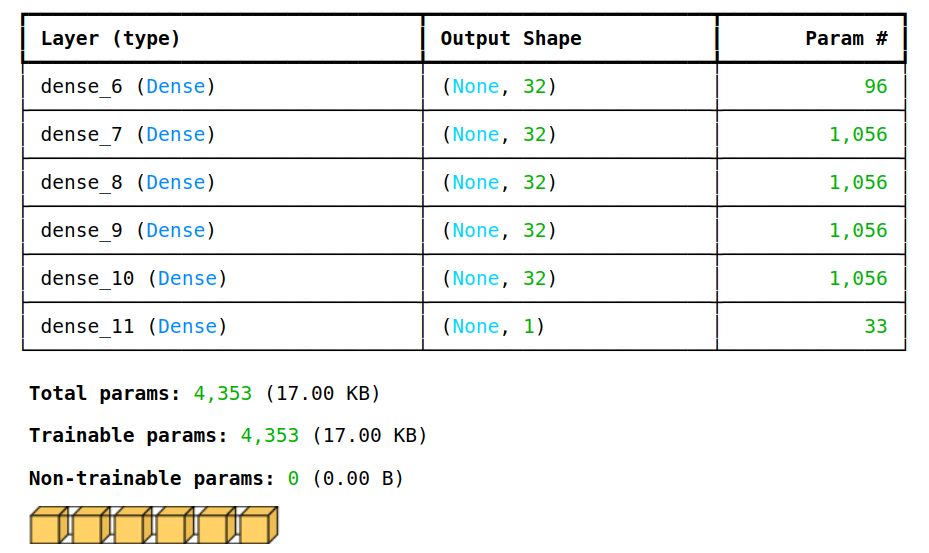
\includegraphics[width=0.9\hsize]{images/visualization_1.png}
\caption{Нейронная сеть - состояние}
\label{fig:error}
\end{figure}

Наша нейронная сеть будет обучена для нахождения функции, которая удовлетворяет этому уравнению, используя соответствующие граничные условия и данные.
Нетренируемых параметров, иначе гиперпараметров нет, потому что коэффициент $\lambda$ мы подбираем сами, тренируя нейросеть с одинаковыми изначальными параметрами в цикле.
